\section{ĐỀ SỐ \thesection } %Đề 20
\setcounter{bt}{0}

%%Câu 1.
\begin{bt} \textbf{ }
	\begin{enumerate}
		\item Tìm tất cả các ước của $-18$.
		\item Tìm số tự nhiên $x$ biết $x\ \vdots \ 28$, $x \ \vdots \ 8$ và $x<300$.
		\item Sắp xếp các số nguyên sau theo thứ tự tăng dần: $2000;-201;0;-199;2024$. 
	\end{enumerate}
	\loigiai{\begin{listEX}[2]
		\item  Ư$(-18)=\{\pm1;\pm2;\pm3;\pm6;\pm9;\pm18\}$ 
		\item $x\in\{0;56;112;168;224;280\}$ 
		\item $-201;-199;0;2000;2024$
		\end{listEX}	}
\end{bt}


%%Câu 2.
\begin{bt} Tính toán hợp lý (nếu có thể):
	\begin{listEX}[2]
			\item $28\cdot(-63)+28\cdot(-37)+800$;
			\item $(-24):(-2)^3+38:(15+4)$;
			\item $400+150:\left( 2^{30}:2^{25}-3^3\right)  $;
			\item $10+\left[ \left( 8^2-48\right) \cdot5+\left( 2^2\cdot10+8\right) \right] :2^4$.
	\end{listEX}
	\loigiai{a) $-2000$ \hfill b) $5$ \hfill c) $430$ \hfill d) $18$.
	}
\end{bt}



%%Câu 3.
\begin{bt} Tìm số nguyên $x$, biết:
	\begin{listEX}[2]
			\item $52:x=-4$;
			\item $(x+7)-15^0=202-19$;
			\item $2^{x+1}\cdot5-8=72$;
			\item $(2x+5)(5^3-123)=-30$.
	\end{listEX}
	\loigiai{a) $x=-13$ \hfill b) $x=177$ \hfill c) $x=3$ \hfill d) $x=-10$.
	}
\end{bt}


%%Câu 4.
\begin{bt} Điểm kiểm tra thường xuyên môn Anh văn của học sinh lớp 6A được cho bởi bảng thống kê sau:
	\begin{center}
		\begin{tabular}{|c|c|c|c|c|c|c|c|c|c|}\hline
			\textbf{Điểm số}&2&3&4&5&6&7&8&9&10 \\ \hline
			\textbf{Số học sinh}&2&1&3&4&5&3&6&8&4 \\ \hline
		\end{tabular}\\
	\end{center}
	\begin{enumerate}
		\item Lớp 7A có tổng cộng bao nhiêu học sinh? 
		\item Điểm số nào có số học sinh đạt được ít nhất? Điểm số nào có số học sinh đạt được nhiều nhất?
		\item Có bao nhiêu học sinh đạt từ điểm 8 trở lên? Chiếm tỷ lệ bao nhiêu phần trăm?
	\end{enumerate}
	\loigiai{a) Có $36$ học sinh \hfill b) Ít nhất: $3$ điểm, nhiều nhất: $9$ điểm \hfill c) Có $18$ học sinh, chiếm $50\%$
	}
\end{bt}


%%Câu 5.
\begin{bt} \immini{Điền các số $ -1$, $ -2$, $-3$, $-4$, $5$, $ 6$, $7$ vào các vòng tròn trên sao cho 
	tổng của ba số nằm trên cùng một hàng thẳng đều bằng $0$.}{
	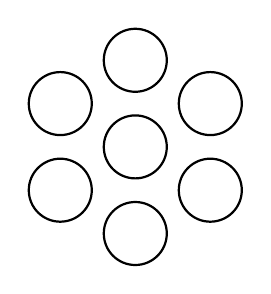
\begin{tikzpicture}[thick,scale=0.5]
		\def\R{2.2}
		\def\r{8mm}
		
		% 6 vòng tròn ngoài
		\foreach \a in {90,30,-30,-90,-150,150}{
			\draw (\a:\R) circle (\r);
		}
		% vòng tròn tâm
		\draw (0,0) circle (\r);
		
		
	\end{tikzpicture}}
	\loigiai{
		\text{}
		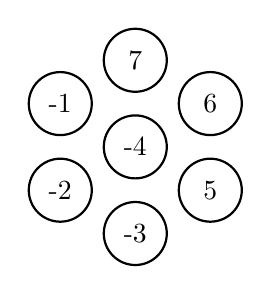
\begin{tikzpicture}[thick,scale=0.5]
			\def\R{2.2}
			\def\r{8mm}
			
			% 6 vòng tròn ngoài
			\foreach \a in {90,30,-30,-90,-150,150}{
				\draw (\a:\R) circle (\r);
			}
			% vòng tròn tâm
			\draw (0,0) circle (\r);
			
			% điền số
			\node at (90:\R) {7};
			\node at (30:\R) {6};
			\node at (-30:\R) {5};
			\node at (-90:\R) {-3};
			\node at (-150:\R) {-2};
			\node at (150:\R) {-1};
			\node at (0,0) {-4};
	\end{tikzpicture}}
\end{bt}



%%Câu 6.
		\begin{bt} 
			\immini[thm]{Một mảnh vườn hình chữ nhật có chiều dài 35 m, chiều rộng là 25 m với lối đi hình bình hành rộng 4 m.
			\begin{enumerate}
				\item Tính diện tích miếng đất hình chữ nhật. 
				\item Tính diện tích phần mảnh vườn không tính lối đi.
			\end{enumerate}
		}{
		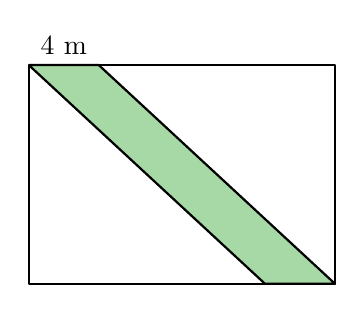
\begin{tikzpicture}[scale=1,line width=0.8pt,line join=round,>=stealth]
			\def\s{9}
			\draw[fill=white] (0,0) rectangle (35/\s,25/\s);
			\draw[fill=green!40!gray!50] (0,25/\s)--(27/\s,0)--(35/\s,0)--(8/\s,25/\s)--(0,25/\s)node[midway,above]{4 m};
			\end{tikzpicture}
		}
			\loigiai{a) $875$ m$^2$ \hfill b) $775$ m$^2$.}
		\end{bt}
		

%%Câu 7.
\begin{bt} Tìm số nguyên $x$ để $(2x+3)\,\vdots\,(x-1)$.
	\loigiai{$n\in\{2;0;6;-4\}$}
\end{bt}